% 2013 年广东卷理科第 15 题：圆 O 的直径 AB，C 在圆上，BC=CD，
% 过 C 的切线与 AD 交于 E，AB=6，ED=2。
% 来源 PDF：普通高考/2013/2013广东理.pdf，第 1 页（印面 803）中栏下部。
% 按计算结果作图：半径 3，BC=2√3，AC=2√6，E 在 AD 上且 AE=4。
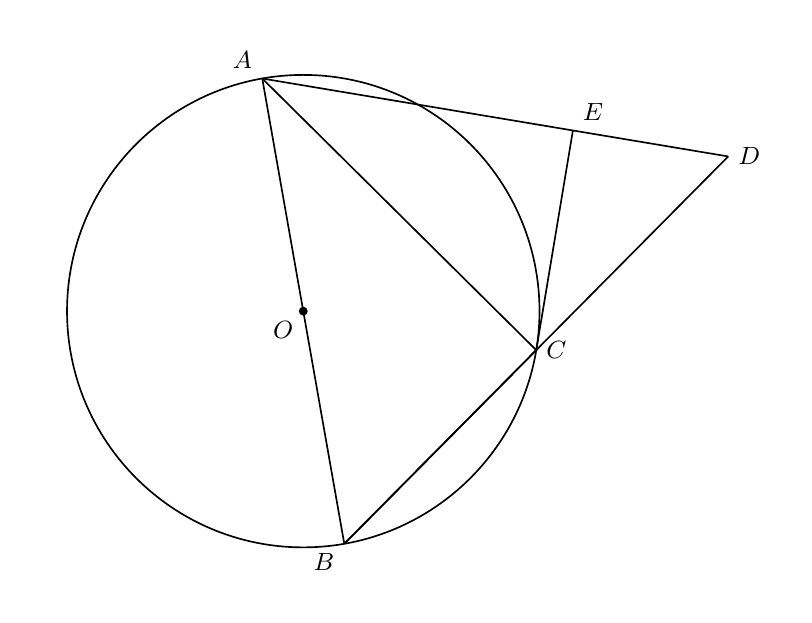
\begin{tikzpicture}[semithick, font=\small]
  \useasboundingbox (-3.5,-3.6) rectangle (6.1,3.6);
  \coordinate (O) at (0,0);
  \coordinate (A) at (-0.5209,2.9544);
  \coordinate (B) at (0.5209,-2.9544);
  \coordinate (C) at (2.9590,-0.4949);
  \coordinate (D) at (5.3971,1.9646);
  \coordinate (E) at (3.4245,2.2945);
  \draw (O) circle[radius=3];
  \draw (A) -- (B);
  \draw (A) -- (C) -- (B);
  \draw (B) -- (D);
  \draw (A) -- (D);
  \draw (C) -- (E);
  \fill (O) circle[radius=1.6pt];
  \node[above left] at (A) {$A$};
  \node[below left] at (B) {$B$};
  \node[right] at (C) {$C$};
  \node[right] at (D) {$D$};
  \node[above right] at (E) {$E$};
  \node[below left] at (O) {$O$};
\end{tikzpicture}
